\documentclass[]{beamer}
\usepackage[utf8]{inputenc}

\title{What is Computing?}
\date{}

\begin{document}

\begin{frame}
    \titlepage
\end{frame}

\begin{frame}{What is a Computer?}

    \begin{columns}
        \begin{column}{0.5\textwidth}
            A "computer" is anything that executes a set of defined instructions.

            \vspace{\baselineskip}

            \begin{itemize}
                \item We will mainly talk about computers that use electrical circuits.
                \item We can assume instructions are executed one at a time in order.
                \item In the common sense of the word, we will be talking about computers like your laptop or desktop computer (or also your phone).
            \end{itemize}
        \end{column}
        \begin{column}{0.5\textwidth}
            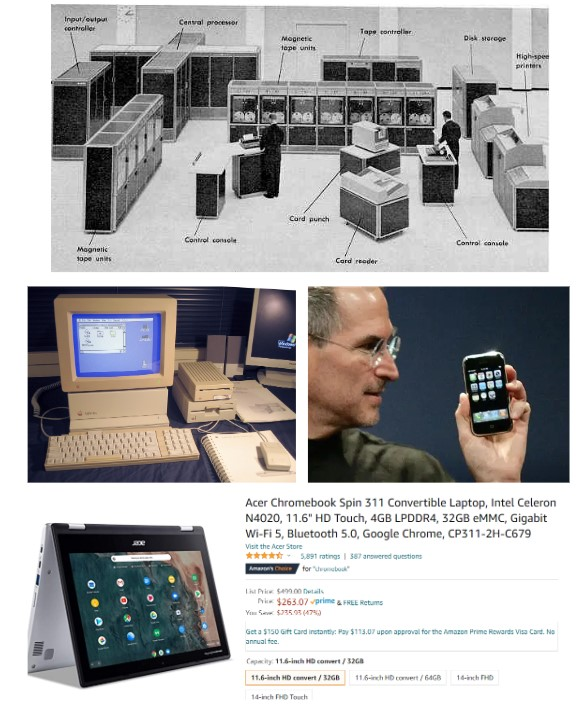
\includegraphics[width=\textwidth]{imgs/vis_0.jpg}
        \end{column}
    \end{columns}
\end{frame}



\end{document}